Dans cette section, nous expliquons dans un premier temps  
le principe du branch and price puis nous détaillons les différentes stratégies de branchements que nous avons trouvées dans la littérature et celle que nous utilisons.

\subsection{Description du branch and price}
La génération de colonnes permet de résoudre des programmes linéaires de grande taille.
Pour pouvoir résoudre des programmes linéaires en nombres entiers il faut ajouter un arbre de branchement.
Lorsque l'on couple la génération de colonnes avec un arbre de branchement on obtient un arbre de branch and price \cite{dantzig1961decomposition,barnhart1998branch}.
Le fonctionnement est le même que pour un arbre de branch and bound sauf que dans le branch and price on résout à chaque n\oe ud le programme linéaire en utilisant la génération de colonnes (c.f. figure~\ref{fig:BP}).
Comme pour le branch and bound, le branch and price permet de conserver la garantie d'optimalité.
Si toutes les branches ont été coupées ou parcourues, alors la solution optimale est la meilleure solution entière obtenue dans un n\oe ud de l'arbre.

\begin{figure}
[H]
\centering
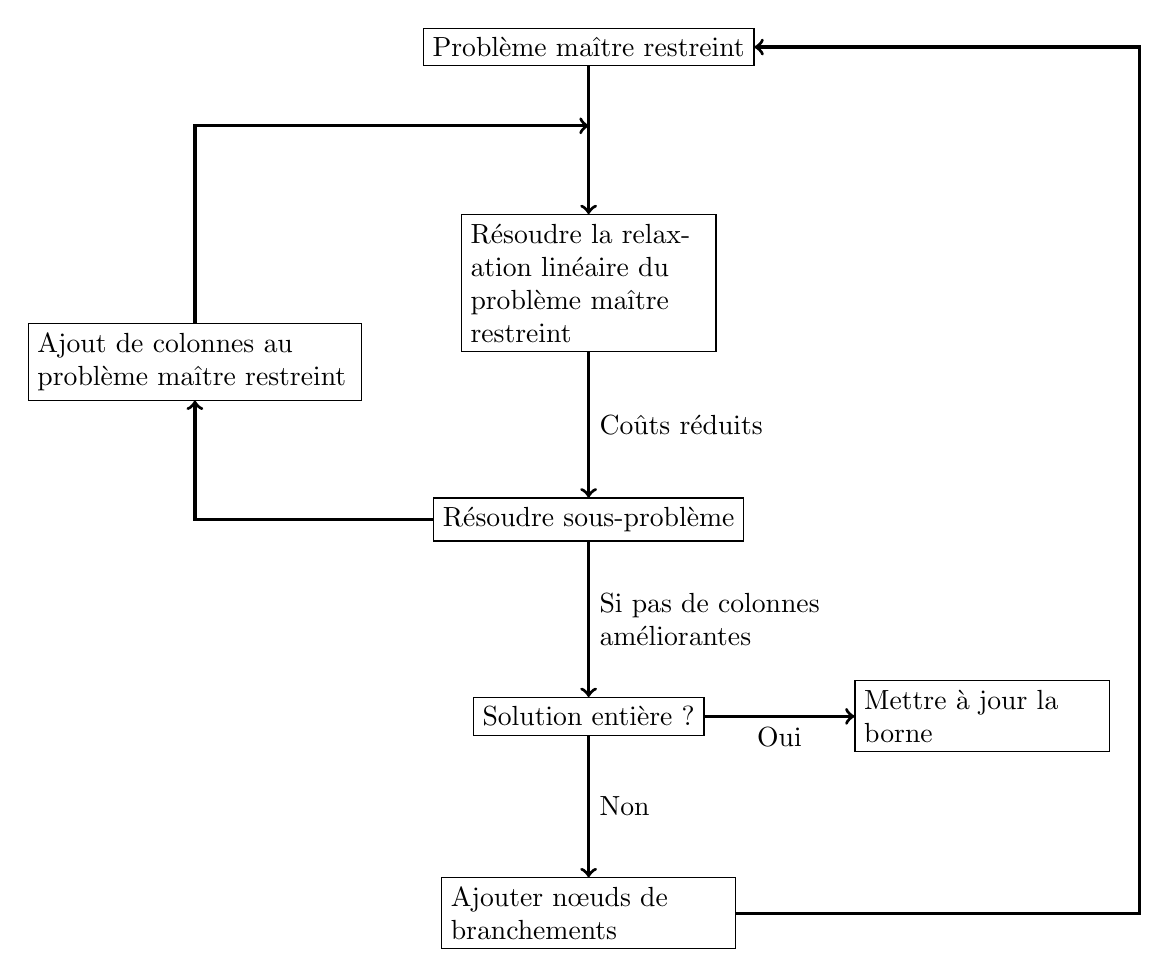
\begin{tikzpicture}

\node[draw,rectangle] (0) at (5,6) {Problème maître restreint};

\node[draw,rectangle,text width=3cm] (1) at (5,3) {Résoudre la relaxation linéaire du problème maître restreint};

\node[draw,rectangle] (2) at (5,0) {Résoudre sous-problème};

\node[draw,rectangle,text width=4cm] (3) at (0,2) {Ajout de colonnes au problème maître restreint};

\node[draw,rectangle] (4) at (5,-2.5) {Solution entière ?};

\node[draw,rectangle,text width=3cm] (5) at (10,-2.5) {Mettre à jour la borne};

\node[draw,rectangle,text width=3.5cm] (6) at (5,-5) {Ajouter nœuds de branchements};

\draw[->,very thick] (0)--(1);
\draw[->,very thick] (1)--(2)node[right,midway]{Coûts réduits};
\draw[->,very thick] (2.west)-|(3.south);
\draw[->,very thick] (3.north)|-(5,5);
\draw[->,very thick] (2)--(4)node[text width=3.5cm,right,midway]{Si pas de colonnes améliorantes};
\draw[->,very thick] (4)--(5)node[midway,below]{Oui};
\draw[->,very thick] (4)--(6)node[midway,right]{Non};
\draw[->,very thick] (6.east)-|(12,-3)|-(0.east);

\end{tikzpicture}
\caption{Figure illustrant le branch and price.\label{fig:BP}}
\end{figure}


\subsection{Les stratégies de branchements}

Pour les stratégies de branchements nous nous sommes inspirés des stratégies présentées dans l'article de Feillet et al. \cite{feillet2010}.
Il présente deux stratégies de branchement : nous appellerons la première : stratégie standard et la seconde : stratégie naturelle.

La stratégie standard correspond au branchement sur les variables de décision du RMP : $\schevar{s}{p}$.
On l'appelle stratégie standard car en général les arbres de branchement utilisent les variables de décisions du programme linéaire associé.

Lorsque la variable $\schevar{s}{p}$ est contrainte à 1 il suffit de sélectionner cette tournée dans le RMP et il faut supprimer tous les sommets présents dans cette tournée dans le PSP.

Cependant lorsqu'elle est contrainte à 0 la tournée n'est pas sélectionnée dans le RMP ($\schevar{s}{p}=0$) et dans le PSP il faut trouver des tournées différentes de cette tournée.
Ce qui implique de calculer les deux meilleurs plus court chemins et plus généralement les $d$ meilleurs plus court chemins lorsqu'il y a $d$ tournées contraintes à 0.

Ce branchement est peu efficace car il ne limite que très peu l'espace de recherche du PSP et du RMP. 
Alors que le branchement avec la variable $\schevar{s}{p}=1$ est plus fort car il permet de se rapprocher d'une solution entière assez rapidement.

La stratégie naturelle correspond au branchement sur les variables de flots $x_{ij}$.
Nous rappelons que $x_{ij}$ indique si la tâche $j$ est effectuée après la tâche $i$.
Cette stratégie est plus naturelle car elle branche sur les variables qui sont connectées à nos tournées.
Ces variables représentent les décisions locales prises par les véhicules.
Cette stratégie est devenue une norme pour les problèmes de tournées de véhicules.
Notons $f_{ij}$ le flot sur l'arc $(i,j)$.
Pour le branchement on choisit un arc $(i,j)$ tel que $0<f_{ij}<1$ ($f_{ij}=\sumP{p} x_{ij}^p$).
Dans ce cas deux branches sont dérivées :
\begin{itemize}
\item Dans une branche, l'arc ne doit pas appartenir à la solution : $f_{ij}=0$.
\item Dans l'autre branche, l'arc doit appartenir à la solution $f_{ij}=1$.
\end{itemize}

Si $f_{ij}$ est contraint à 1 alors dans le PSP les arcs $(i,k),~\forall k\not=j$ et  $(k,j),~\forall k\not=i$ doivent être supprimés.
Toutes les tournées générées passeront soit par l'arc $(i,j)$, soit ne passeront ni par $i$ ni par $j$ car c'est le seul arc sortant pour $i$ et entrant pour $j$.
Dans le RMP, il faut supprimer toutes les tournées telles que : les tournées passent par un des arcs $(i,k),~\forall k\not=j$ et  $(k,j),~\forall k\not=i$.
De plus il faut forcer les tâches $i$ et $j$ à être exécutées : $\gamma_i=0$ et $\gamma_j=0$.
Les tâches $i$ et $j$ appartiennent forcément à la solution et comme tous les autres arcs ont été supprimés : $i$ est directement suivit de $j$ (l'arc $(i,j)$ appartient aussi à la solution).

Si $f_{ij}$ est contraint à 0 alors dans le PSP l'arc $(i,j)$ est supprimé. 
Aucune tournée générée avec le PSP ne contiendra l'arc $(i,j)$.
Dans le RMP, il faut supprimer toutes les tournées passant par l'arc $(i,j)$.
Ainsi $f_{ij}=0$ car aucune tournée ne passera par $j$ directement après $i$.

Ce branchement se base sur le fait que les tournées appartenant à une solution réalisable sont disjointes.
Dans le graphe représentant les tournées, tous les sommets (tâches) ont un degré deux.
Ainsi le flot sur un arc pour toute tournée est $0< f_{ij}<1$.
Cependant si les tâches peuvent être visitées plusieurs fois dans les solutions optimales alors cette stratégie de branchement est difficilement transposable car brancher sur certains arcs couperait des solutions optimales.


Il existe cependant d'autres stratégies de branchement comme par exemple la stratégie de branchement sur les fenêtres temporelles ou sur les contraintes de précédence.
Nous n'avons pas décidé d'implémenter ces stratégies car dans les instances que nous traitons il y a peu de contraintes de précédence. 
La stratégie sur les fenêtres temporelles nous semble peu efficace sur nos instances car le fait qu'il y ait plusieurs fenêtres temporelles fait qu'un branchement sur celles-ci ne converge que très peu vers une solution réalisable.


\subsection{Les stratégies de parcours de l'arbre de branchements}

L'arbre de branchements représente l'espace des solutions.
Son parcours est donc très important pour obtenir la solution optimale avec le moins de temps possible.
Il existe différentes stratégies de recherche dans un arbre parcours : parcours en profondeur (depth-first search en anglais), parcours en largeur (breadth-first search en anglais) et parcours du "meilleur d'abord" (best-first search en anglais).

Le parcours en profondeur vise à obtenir une solution entière rapidement, puis parcours l'arbre pour essayer d'améliorer cette solution entière.
Le n\oe ud le plus profond dans l'arbre est sélectionné en premier.
Comme cette solution donne une borne, cette stratégie permet de couper de nombreuses branches.

Le parcours en largeur permet de parcourir l'arbre dans sa totalité niveau par niveau. 
La racine étant au niveau 0, ses voisins au niveau 1 et ainsi de suite ...
Cette stratégie n'est pas efficace car elle demande de stocker en mémoire tous les n\oe uds d'un niveau de l'arbre.

Le parcours "meilleur d'abord" permet d'obtenir une solution entière de bonne qualité, il est même probable que cette solution soit optimale.
Le n\oe ud avec la meilleure solution relâchée est sélectionné en premier.
Jusqu'à l'obtention de cette solution aucune branche ne sera coupée.
Cependant lorsque cette solution est trouvée la plupart des branches seront coupées.

Il est aussi possible de coupler certain parcours entre eux comme par exemple : le parcours en profondeur et le parcours "meilleur d'abord" : les n\oe uds les plus profonds dans l'arbre sont gardés puis celui qui à la meilleure solution relâchée est sélectionné.




